%% LyX 2.3.7 created this file.  For more info, see http://www.lyx.org/.
%% Do not edit unless you really know what you are doing.
\documentclass[10pt,english,t,10pt,handout]{beamer}
\usepackage{lmodern}
\usepackage[T1]{fontenc}
\usepackage[utf8]{inputenc}
\setcounter{tocdepth}{1}
\setlength{\parskip}{\smallskipamount}
\setlength{\parindent}{0pt}
\usepackage{babel}
\usepackage{amsbsy}
\usepackage{amstext}
\usepackage{graphicx}
\usepackage[authoryear]{natbib}
\ifx\hypersetup\undefined
\AtBeginDocument{%
\hypersetup{unicode=true}
}
\else
\hypersetup{unicode=true}
\fi
\makeatletter
%%%%%%%%%%%%%%%%%%%%%%%%%%%%%% Textclass specific LaTeX commands.
% this default might be overridden by plain title style
\newcommand\makebeamertitle{\frame{\maketitle}}%
% (ERT) argument for the TOC
\AtBeginDocument{%
\let\origtableofcontents=\tableofcontents
\def\tableofcontents{\@ifnextchar[{\origtableofcontents}{\gobbletableofcontents}}
\def\gobbletableofcontents#1{\origtableofcontents}
}
%%%%%%%%%%%%%%%%%%%%%%%%%%%%%% User specified LaTeX commands.
\usepackage{tikz}
\usetikzlibrary{positioning}
\usepackage{appendixnumberbeamer}
\usepackage{graphicx}
\usepackage{subfig}
\usetheme[progressbar=frametitle,block=fill,subsectionpage=progressbar]{metropolis}
% margin
\setbeamersize{text margin right=1.5cm}
% colors
\definecolor{DarkRed}{rgb}{0.7,0,0}
%\colorlet{DarkRed}{redblack}
\setbeamercolor{normal text}{fg=black}
\setbeamercolor{alerted text}{fg=DarkRed}
\setbeamercolor{progress bar}{fg=DarkRed}
\setbeamercolor{button}{bg=DarkRed}
% width of seperators
\makeatletter
\setlength{\metropolis@titleseparator@linewidth}{1pt}
\setlength{\metropolis@progressonsectionpage@linewidth}{1pt}
\setlength{\metropolis@progressinheadfoot@linewidth}{1pt}
\makeatother
% new alert block
\newlength\origleftmargini
\setlength\origleftmargini\leftmargini
\setbeamertemplate{itemize/enumerate body begin}{\setlength{\leftmargini}{4mm}}
\let\oldalertblock\alertblock
\let\oldendalertblock\endalertblock
\def\alertblock{\begingroup \setbeamertemplate{itemize/enumerate body begin}{\setlength{\leftmargini}{\origleftmargini}} \oldalertblock}
\def\endalertblock{\oldendalertblock \endgroup}
\setbeamertemplate{mini frame}{}
\setbeamertemplate{mini frame in current section}{}
\setbeamertemplate{mini frame in current subsection}{}
\setbeamercolor{section in head/foot}{fg=normal text.bg, bg=structure.fg}
\setbeamercolor{subsection in head/foot}{fg=normal text.bg, bg=structure.fg}
% footer
\makeatletter
\setbeamertemplate{footline}{%
\begin{beamercolorbox}[colsep=1.5pt]{upper separation line head}
\end{beamercolorbox}
\begin{beamercolorbox}{section in head/foot}
\vskip1pt\insertsectionnavigationhorizontal{\paperwidth}{}{\hskip0pt plus1filll \insertframenumber{} / \inserttotalframenumber \hskip2pt}\vskip3pt% 
\end{beamercolorbox}%
\begin{beamercolorbox}[colsep=1.5pt]{lower separation line head}
\end{beamercolorbox}
}
\makeatother
% toc
\setbeamertemplate{section in toc}{\hspace*{1em}\inserttocsectionnumber.~\inserttocsection\par}
\setbeamertemplate{subsection in toc}{\hspace*{2em}\inserttocsectionnumber.\inserttocsubsectionnumber.~\inserttocsubsection\par}
\makeatother
\begin{document}
\title{4. Transition Path\vspace{-2mm}}
\subtitle{Adv. Macro: Heterogenous Agent Models} 
\author{Nicolai Waldstrøm}
\date{2024}
{
\setbeamertemplate{footline}{} 
\begin{frame}
\maketitle
\begin{tikzpicture}[overlay, remember picture]
\node[above left=0cm and 0.0cm of current page.south east] 
{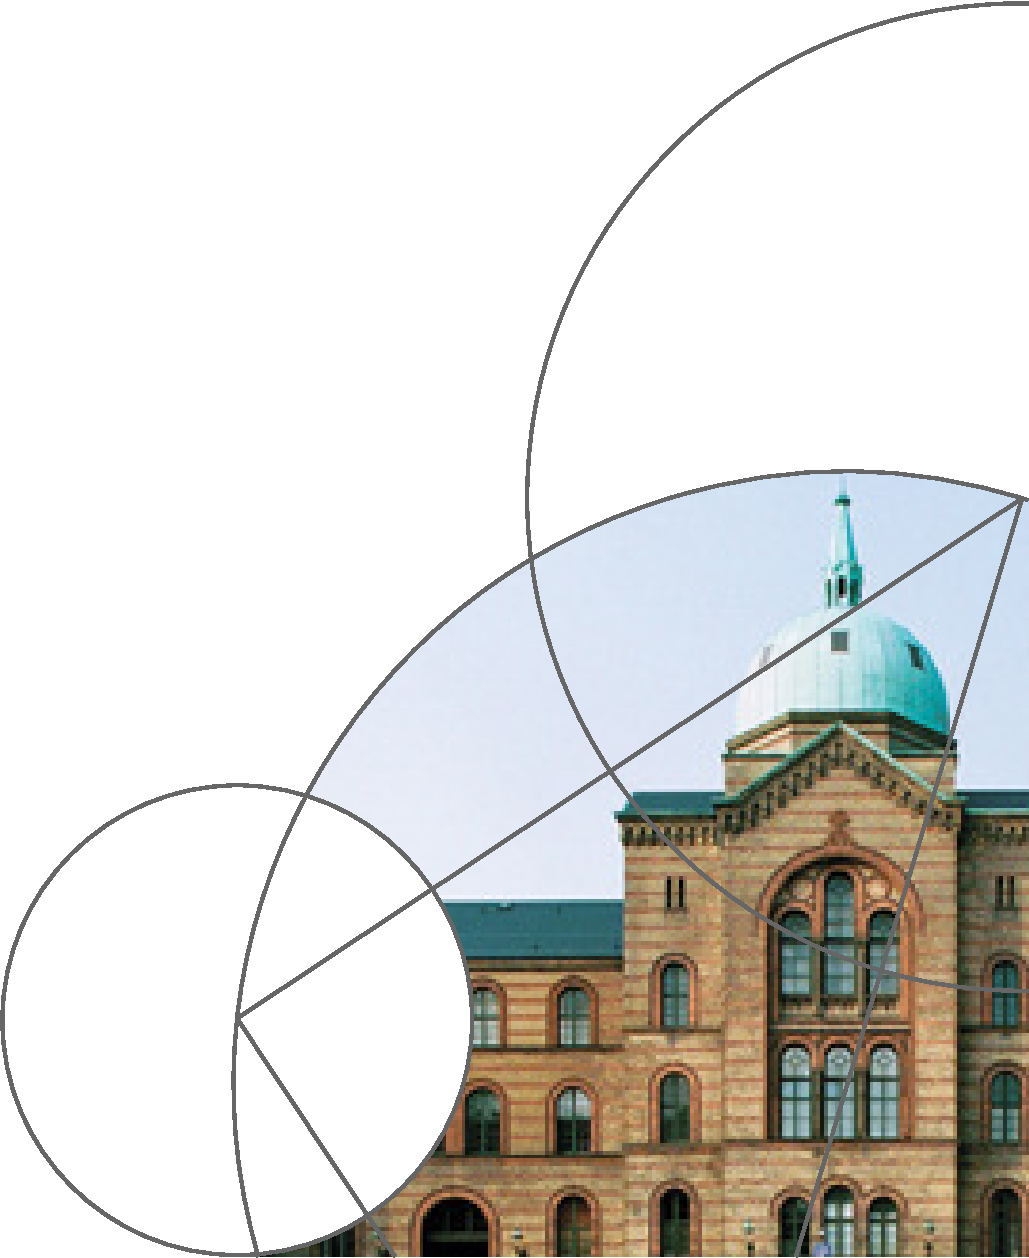
\includegraphics[width=4cm]{figs/KUSAMFtitlelrcorner.pdf}};
\end{tikzpicture}
\begin{tikzpicture}[overlay, remember picture]
\node[below left=0.5cm and .8cm of current page.north east] 
{\includegraphics[width=1.5cm]{figs/KUSAMFlogo.pdf}};
\end{tikzpicture}
\end{frame}
}
\addtocounter{framenumber}{-1}
\section{Introduction}
\begin{frame}{Introduction}
\vspace{-2mm}
\begin{itemize}
\item <+->\textbf{Last time: }\emph{Stationary equilibrium (steady states)}
\item <+->\textbf{Today:} \emph{Transition path (dynamic responses away
from steady state)}
\item <+->\textbf{Model:} Heterogeneous Agent Neo-Classical (HANC) model
\item <+->\textbf{Code:} 
\begin{enumerate}
\item Based on the \textcolor{DarkRed}{\href{https://github.com/NumEconCopenhagen/GEModelTools}{GEModelTools}}
package
\item Example from \textcolor{DarkRed}{\href{https://github.com/NumEconCopenhagen/GEModelToolsNotebooks}{GEModelToolsNotebooks/HANC}}\\
(except stuff on \emph{linearized solution} and \emph{simulation})
\end{enumerate}
\item <+->\textbf{Literature: }
\begin{enumerate}
\item Auclert et. al. (2021), >>Using the Sequence-Space Jacobian to Solve
and Estimate Heterogeneous-Agent Models<<
\item Documentation for GEModelTools\\
(except stuff on \emph{linearized solution} and \emph{simulation})
\item Kirkby (2017)
\end{enumerate}
\end{itemize}
\end{frame}
%
\begin{frame}{Example I }
\begin{itemize}
\item What do we mean by transition path?
\item Permanent shock to labor supply (think increase in retirement age)
in the macroeconomic model of the Ministry of Finance: \vspace{1cm}\\
\begin{figure}[H]     \centering     
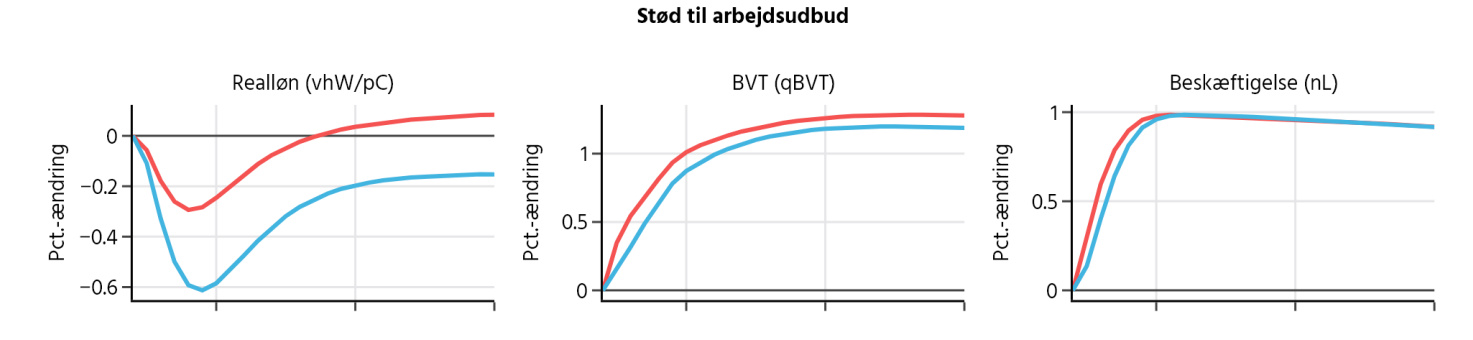
\includegraphics[width=0.99\linewidth]{figs/MAKRO_ex1.png}     
\end{figure}
\item \vspace{1cm}Note: Permanent shock, so transition path \emph{between}
two different steady states
\end{itemize}
\end{frame}
%
\begin{frame}{Example II}
\begin{itemize}
\item Temporary shock to public spending (i.e. fiscal stimulus during recessions)\\
\begin{figure}[H]     \centering     
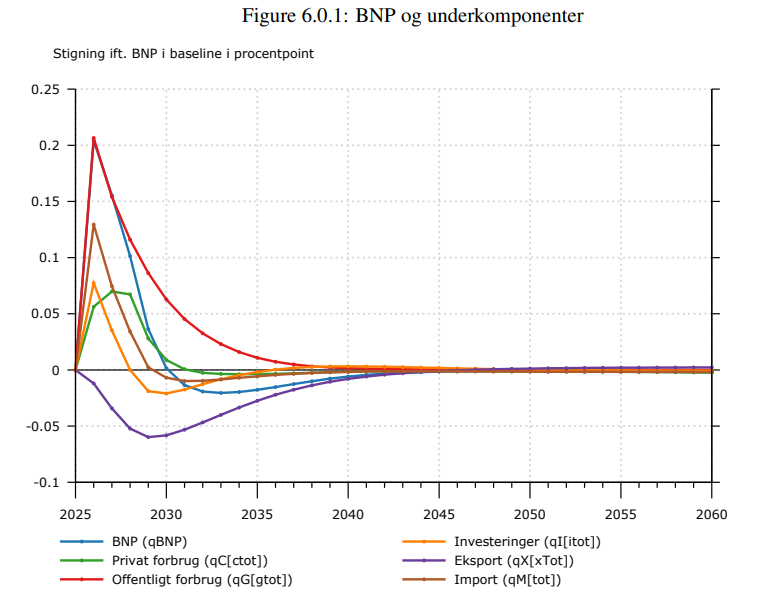
\includegraphics[width=0.7\linewidth]{figs/MAKRO_ex2.png}     
\end{figure}
\item Note: Temporary shock, so model returns to the \emph{same steady state}
\end{itemize}
\end{frame}
%
\section{Standard Ramsey model}
\begin{frame}{Ramsey: Summary}
\begin{itemize}
\item \textbf{Simplified form:}
\begin{align*}
u^{\prime}(C_{t}^{hh}) & =\beta(1+F_{K}(K_{t},1)-\delta)u^{\prime}(C_{t+1}^{hh})\\
K_{t} & =(1-\delta)K_{t-1}+F(K_{t-1},1)-C_{t}^{hh}
\end{align*}
\item \textbf{Production function:} $\Gamma_{t}K_{t}^{\alpha}L_{t}^{1-\alpha}$
\item \textbf{Utility function:} $\frac{\left(C_{t}^{hh}\right)^{1-\sigma}}{1-\sigma}$
\item \textbf{Steady state:
\begin{align*}
K_{ss} & =\left(\frac{\left(\frac{1}{\beta}-1+\delta\right)}{\Gamma_{ss}\alpha}\right)^{\frac{1}{\alpha-1}}\\
C_{ss}^{hh} & =(1-\delta)K_{ss}+\Gamma_{ss}K_{ss}^{\alpha}-K_{ss}
\end{align*}
}
\end{itemize}
\end{frame}
%
\begin{frame}{Ramsey: As an equation system}
\begin{align*}
\left[\begin{array}{c}
r_{t}^{K}-\alpha\Gamma_{t}K_{t}^{\alpha-1}L_{t}^{1-\alpha}\\
w_{t}-(1-\alpha)\Gamma_{t}K_{t}^{\alpha}L_{t}^{-\alpha}\\
r_{t}-(r_{t}^{K}-\delta)\\
A_{t}-K_{t}\\
A_{t}^{hh}-\left((1+r_{t})A_{t-1}^{hh}+w_{t}L_{t}^{hh}-C_{t}^{hh}\right)\\
C_{t}^{hh,-\sigma}-\beta(1+r_{t+1})C_{t+1}^{hh,-\sigma}\\
A_{t}-A_{t}^{hh}\\
L_{t}-L_{t}^{hh}\\
\forall t\in\{0,1,\dots\},\text{given }K_{-1}
\end{array}\right] & \boldsymbol{=}\boldsymbol{0}
\end{align*}
\textbf{Remember:} Perfect foresight w.r.t aggregate variables\\
\textbf{Unknowns}: $\{r_{t}^{K},w_{t},L_{t},K_{t},r_{t},A_{t},C_{t}^{hh},A_{t}^{hh}\}$
for $\forall t\in\{0,1,\dots\}$
\end{frame}
%
\begin{frame}{Recap: Newton's method I}
\begin{itemize}
\item <+->Before solving the dynamic Ramsey model, consider a simpler example 
\item <+->Want to solve 1 eq. with 1 unknown (x is a scalar):
\[
f\left(x\right)=0
\]
\item <+->\textbf{How to find} x? First-order Taylor approximation around
current guess $x^{i}$:
\[
f\left(x\right)\approx f\left(x^{i}\right)+f'\left(x^{i}\right)\left(x-x^{i}\right)
\]
\item <+->Set $f\left(x\right)=0$ and solve for x to get:
\[
x=x^{i}-\frac{f\left(x^{i}\right)}{f'\left(x^{i}\right)}
\]
\end{itemize}
\end{frame}
%
\begin{frame}{Recap: Newton's method II }
\begin{itemize}
\item <+->Newton's method: Given initial guess $x_{0}$ update guess for
$x$ from $i$ to $i+1$ as:
\[
x^{i+1}=x^{i}-\frac{f\left(x^{i}\right)}{f'\left(x^{i}\right)}
\]
\begin{itemize}
\item until $\left|f\left(x^{i}\right)\right|<\epsilon$
\end{itemize}
\item <+->Can always get $f\left(x^{i}\right)$ by simply evaluating the
function at current estimate. What about derivative $f'\left(x^{i}\right)$?
\item <+->Use numerical approximation:
\[
f'\left(x^{i}\right)\approx\frac{f\left(x^{i}+h\right)-f\left(x^{i}\right)}{h}
\]
\begin{itemize}
\item For small $h$.
\end{itemize}
\item <+->How well does it work?
\begin{itemize}
\item If $f\left(x\right)$ is linear this update solves $f\left(x\right)=0$
in \textbf{1 iteration}
\item If $f\left(x\right)$ is non-linear we typically need more iterations,
but works well if initial guess is within basis of attraction
\end{itemize}
\end{itemize}
\end{frame}
%
\begin{frame}{Recap: Multivariate Newton's method}
\begin{itemize}
\item <+->Generalize to vector-valued, multivariate functions $\left[f_{1}\left(x_{1,}x_{2}\right),f_{2}\left(x_{1,}x_{2}\right)\right]'=\boldsymbol{f}\left(\boldsymbol{x}\right)$
with $\boldsymbol{x}=\left(x_{1,}x_{2}\right)'$ :
\[
\boldsymbol{x}^{i+1}=\boldsymbol{x}^{i}-\boldsymbol{J}\left(\boldsymbol{x}^{i}\right)^{-1}\boldsymbol{f}\left(\boldsymbol{x}^{i}\right)
\]
\item <+->Where $\boldsymbol{J}\left(\boldsymbol{x}^{i}\right)$ is the
\emph{Jacobian }of\emph{ $f\left(\boldsymbol{x}\right)$ }w.r.t $\boldsymbol{x}^{i}$:
\[
\boldsymbol{J}\left(\boldsymbol{x}_{i}\right)=\left[\begin{array}{cc}
\frac{\partial f_{1}}{\partial x_{1}^{i}} & \frac{\partial f_{1}}{\partial x_{2}^{i}}\\
\frac{\partial f_{2}}{\partial x_{1}^{i}} & \frac{\partial f_{2}}{\partial x_{2}^{i}}
\end{array}\right]
\]
\item <+->Can calculate this jacobian in the same way as $f'\left(x\right)$
in previous example, but need to so for every element in \textbf{$\boldsymbol{x}$}
\item <+->\textbf{Go through code}
\end{itemize}
\end{frame}
%
\begin{frame}{Recap: Broyden's method I}
\begin{itemize}
\item <+->Newton's method updates Jacobian $\boldsymbol{J}$ in \textbf{every
iteration}
\item <+->If $\boldsymbol{J}$ is expensive to calculate, this is a serious
bottleneck 
\item <+->Broyden's method solves this issue by only calculating $J$ around
some initial point.
\item <+->Then apply following (linear) update of $f'\left(x^{i+1}\right)$
at every iteration $i$:
\[
f'\left(x^{i+1}\right)=f'\left(x^{i}\right)+\frac{\left[f\left(x^{i+1}\right)-f\left(x^{i}\right)\right]-f'\left(x^{i}\right)\left(x^{i+1}-x^{i}\right)}{x^{i+1}-x^{i}}
\]
\end{itemize}
\end{frame}
%
\begin{frame}{Recap: Broyden's method II}
\begin{enumerate}
\item Guess $\boldsymbol{x}^{0}$ and set $i=0$
\item Calculate the Jacobian around initial point $\boldsymbol{J}_{\boldsymbol{0}}$
\item Calculate $\boldsymbol{f}^{i}=\boldsymbol{f}(\boldsymbol{x}^{i})$.
\item Stop if $\left|\boldsymbol{f}^{i}\right|$ below tolerance $\epsilon$
\item Calculate Jacobian by $\boldsymbol{J}^{i}=\begin{cases}
\boldsymbol{J}_{\boldsymbol{0}} & \text{if }i=0\\
\boldsymbol{J}^{i-1}+\frac{(\boldsymbol{f}^{i}-\boldsymbol{f}^{i-1})-\boldsymbol{J}^{i-1}(\boldsymbol{x}^{i}-\boldsymbol{x}^{i-1})}{\left|\boldsymbol{x}^{i}-\boldsymbol{x}^{i-1}\right|_{2}}\left(\boldsymbol{x}^{i}-\boldsymbol{x}^{i-1}\right)^{\prime} & \text{if }i>0
\end{cases}$
\item Update guess by $\boldsymbol{x}^{i+1}=\boldsymbol{x}^{i}-\left(\boldsymbol{J}^{i}\right)^{-1}\boldsymbol{f}^{i}$
\item Increment $i$ and return to step 3
\end{enumerate}
\begin{itemize}
\item \textbf{Go through code}
\end{itemize}
\end{frame}
%
\begin{frame}{Back to Ramsey}
\begin{align*}
\left[\begin{array}{c}
r_{t}^{K}-\alpha\Gamma_{t}K_{t}^{\alpha-1}L_{t}^{1-\alpha}\\
w_{t}-(1-\alpha)\Gamma_{t}K_{t}^{\alpha}L_{t}^{-\alpha}\\
r_{t}-(r_{t}^{K}-\delta)\\
A_{t}-K_{t}\\
A_{t}^{hh}-\left((1+r_{t})A_{t-1}^{hh}+w_{t}L_{t}^{hh}-C_{t}^{hh}\right)\\
C_{t}^{hh,-\sigma}-\beta(1+r_{t+1})C_{t+1}^{hh,-\sigma}\\
A_{t}-A_{t}^{hh}\\
L_{t}-L_{t}^{hh}\\
\forall t\in\{0,1,\dots\},\text{given }K_{-1}
\end{array}\right] & \boldsymbol{=}\boldsymbol{0}
\end{align*}
\begin{itemize}
\item <+->2 issues:
\begin{itemize}
\item <+->Many unknowns (8 eqs per period)
\item <+->In fact, infinitely many since time is infinite, $T\rightarrow\infty$
\end{itemize}
\end{itemize}
\end{frame}
%
\begin{frame}{Truncated Ramsey, reduced vector form}
\vspace{-7mm}
\begin{align*}
\boldsymbol{H}\left(\boldsymbol{K},\boldsymbol{L},\boldsymbol{\Gamma},K_{-1}\right) & =\left[\begin{array}{c}
A_{t}-A_{t}^{hh}\\
L_{t}-L_{t}^{hh}\\
\forall t\in\{0,1,\dots,T-1\}
\end{array}\right]=\boldsymbol{0}
\end{align*}
where $\boldsymbol{X}=(X_{0},X_{1},\dots,X_{T-1})$, $A_{-1}^{hh}=K_{-1}$
and{\small{}
\begin{align*}
r_{t}^{K} & =\alpha\Gamma_{t}(K_{t-1}/L_{t})^{\alpha-1}\\
w_{t} & =(1-\alpha)\Gamma_{t}(K_{t-1}/L_{t})^{\alpha}\\
A_{t} & =K_{t}\\
r_{t} & =r_{t}^{K}-\delta\\
C_{t}^{hh} & =\left(\beta(1+r_{t+1})\right)^{-\sigma}C_{t+1}^{hh}\,\text{(backwards)}\\
L_{t}^{hh} & =1\\
A_{t}^{hh} & =(1+r_{t})A_{t-1}^{hh}+w_{t}L_{t}^{hh}-C_{t}^{hh}\,\text{(forwards)}
\end{align*}
}\textbf{Truncation:} $T<\infty$ fine when $\Gamma_{t}=\Gamma_{ss}$
for all $t>\underline{t}$ with $\underline{t}\ll T$
\end{frame}
%
\begin{frame}{Further reduced}
\vspace{-7mm}
\begin{align*}
\boldsymbol{H}\left(\boldsymbol{K},\boldsymbol{\Gamma},K_{-1}\right) & =\left[\boldsymbol{A}-\boldsymbol{A}^{hh}\right]=\boldsymbol{0}
\end{align*}
where $\boldsymbol{X}=(X_{0},X_{1},\dots,X_{T-1})$, $A_{-1}^{hh}=K_{-1}$
and{\small{}
\begin{align*}
L_{t}=L_{t}^{hh} & =1\\
r_{t}^{K} & =\alpha\Gamma_{t}(K_{t-1}/L_{t})^{\alpha-1}\\
w_{t} & =(1-\alpha)\Gamma_{t}(K_{t-1}/L_{t})^{\alpha}\\
A_{t} & =K_{t}\\
r_{t} & =r_{t}^{K}-\delta\\
C_{t}^{hh} & =\left(\beta(1+r_{t+1})\right)^{-\sigma}C_{t+1}^{hh}\,\text{(backwards)}\\
A_{t}^{hh} & =(1+r_{t})A_{t-1}^{hh}+w_{t}L_{t}^{hh}-C_{t}^{hh}\,\text{(forwards)}
\end{align*}
}{\small\par}
for $\forall t\in\{0,1,\dots,T-1\}$
\end{frame}
%
\begin{frame}{Sequence space}
\begin{itemize}
\item <+->Note: We have now written the model in \emph{sequence space}
\begin{itemize}
\item Representing an entire timepath/\emph{sequence} of variables as a
function of timepath\emph{/sequence} of other variables
\end{itemize}
\item <+->Example: Keynesian consumption function $C_{t}=a+bY_{t}$:
\begin{align*}
\left[\begin{array}{cccc}
C_{0} & C_{1} & C_{2} & \ldots\end{array}\right]' & =a+b\left[\begin{array}{cccc}
Y_{0} & Y_{1} & Y_{2} & \ldots\end{array}\right]'\\
\Leftrightarrow\boldsymbol{C} & =a+b\boldsymbol{Y}\\
\Leftrightarrow\boldsymbol{C} & =f\left(\boldsymbol{Y}\right)
\end{align*}
\item <+->Powerfull since it also applies \emph{non-linear}, forward-looking
and backwards-looking eqs:
\begin{align*}
C_{t} & =a+b_{0}Y_{t}+b_{1}\log Y_{t-4}+b_{2}Y_{t+4}^{2}\\
\Leftrightarrow\boldsymbol{C} & =g\left(\boldsymbol{Y}\right)
\end{align*}
\item <+->As long as we have the sequence $\boldsymbol{Y}$ we can calculate
$\boldsymbol{C}$
\begin{itemize}
\item Will leverage this later when working with the HA model 
\end{itemize}
\end{itemize}
\end{frame}
%
\begin{frame}{Solution in sequence space}
\begin{itemize}
\item \textbf{Truncation:} $T=200$ (transition path should have converged
to ss by then)
\item \textbf{Jacobian:} Find $\boldsymbol{H}_{\boldsymbol{K}}$ by \emph{numerical
differentiation}
\[
\boldsymbol{H}_{\boldsymbol{K}}=\left[\begin{array}{ccc}
\frac{\partial(A_{0}-A_{0}^{hh})}{\partial K_{0}} & \frac{\partial(A_{0}-A_{0}^{hh})}{\partial K_{1}} & \cdots\\
\frac{\partial(A_{1}-A_{1}^{hh})}{\partial K_{0}} & \ddots & \ddots\\
\vdots & \ddots & \ddots
\end{array}\right]
\]
\item \textbf{Transition path:} Given $\boldsymbol{\Gamma}$ and $K_{-1}$
solve $\boldsymbol{H}\left(\boldsymbol{K},\boldsymbol{\Gamma},K_{-1}\right)$
with non-linear equation system solver (e.g. broyden)
\item \textbf{Notebook:} \emph{Ramsey.ipynb}
\end{itemize}
\end{frame}
%
\begin{frame}{Example 1: Initially low capital}
\textbf{Initially away from steady state: $K_{-1}=0.75K_{ss}$}
\textbf{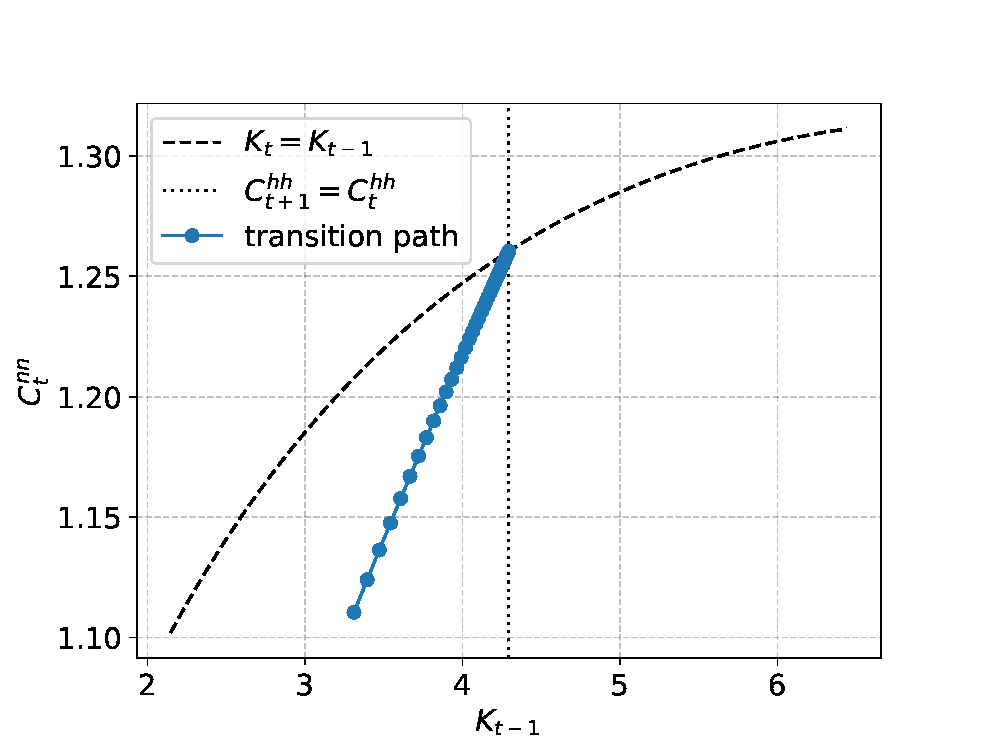
\includegraphics[width=0.8\textwidth]{figs/K_ini_lag}}
\end{frame}
%
\begin{frame}{Example 2: Technology shock}
\textbf{Technology shock: $\Gamma_{t}=0.01\times\Gamma_{ss}\times0.95^{t}$
}(i.e AR(1) with $\rho=0.95$) (exogenous, deterministic)
\textbf{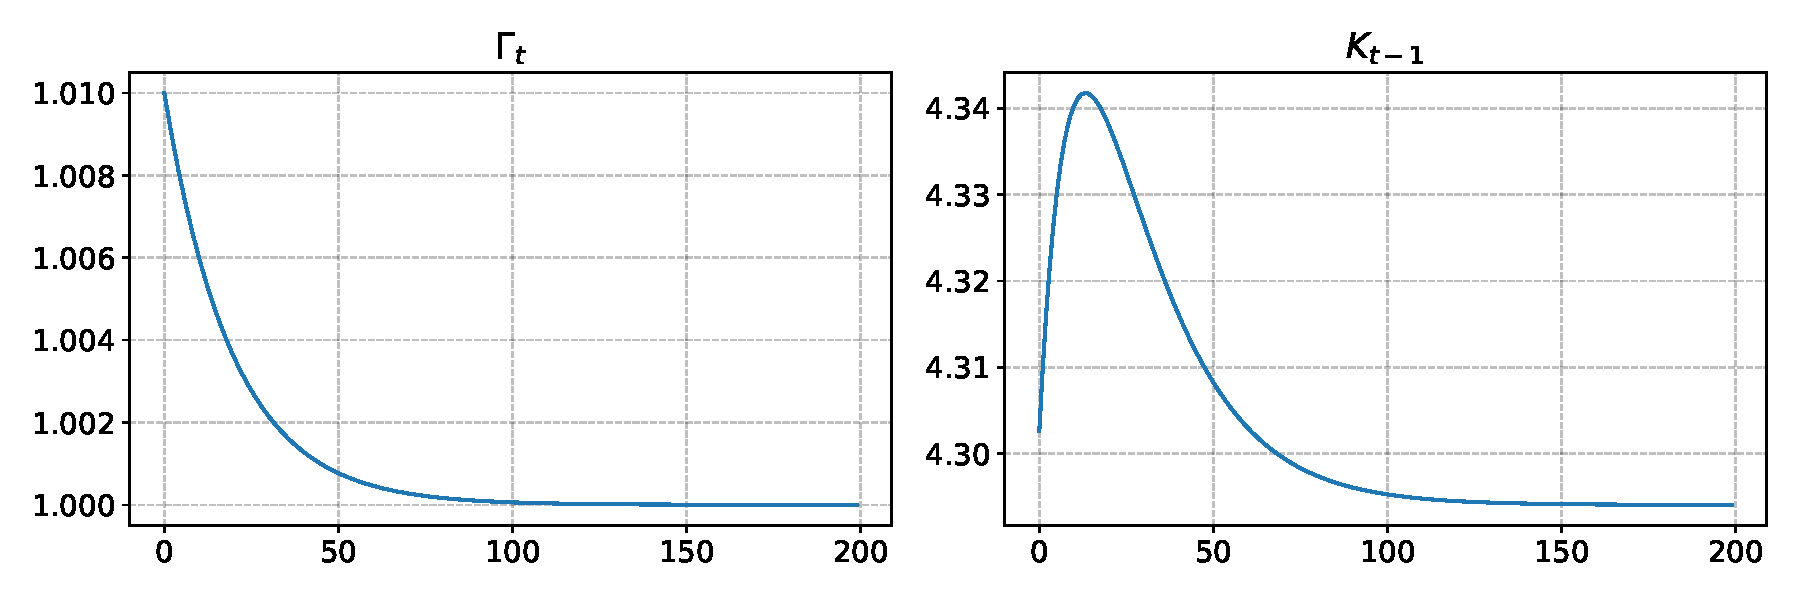
\includegraphics[width=0.95\textwidth]{figs/Gamma_shock}}
\textbf{Terminology:} MIT-shock
\end{frame}
%
\section{Transition path with HA}
\begin{frame}{Equation system}
The model can be written as an \textbf{equation system}{\footnotesize{}
\begin{align*}
\left[\begin{array}{c}
r_{t}^{K}-F_{K}(K_{t-1},L_{t})\\
w_{t}-F_{L}(K_{t-1},L_{t})\\
r_{t}-(r_{t}^{K}-\delta)\\
A_{t}-K_{t}\\
\boldsymbol{D}_{t}-\Pi_{z}\underline{\boldsymbol{D}}_{t}\\
\underline{\boldsymbol{D}}_{t+1}-\Lambda_{t}\boldsymbol{D}_{t}\\
A_{t}-A_{t}^{hh}\\
L_{t}-L_{t}^{hh}\\
\forall t\in\{0,1,\dots\},\text{given }\underline{\boldsymbol{D}}_{0}
\end{array}\right] & =\boldsymbol{0}
\end{align*}
}where $\left\{ \Gamma_{t}\right\} _{t\geq0}$ is a given technology
path and $K_{-1}=\int a_{t-1}d\underline{\boldsymbol{D}}_{0}$
\textbf{Remember: }Policies and choice transitions depend on prices
\begin{enumerate}
\item Policy function: $x_{t}^{\ast}=x^{\ast}\left(\left\{ r_{\tau},w_{\tau}\right\} _{\tau\geq t}\right)$
and $X_{t}^{hh}=\sum_{i}x_{it}^{\ast}D_{it}=\boldsymbol{x}_{t}^{\ast\prime}\boldsymbol{D}_{t}$
\item Choice transition: $\Lambda_{t}=\Lambda\left(\left\{ r_{\tau},w_{\tau}\right\} _{\tau\geq t}\right)$
\end{enumerate}
\end{frame}
%
\begin{frame}{Transition path - close to verbal definition}
{\small{}For a given $\boldsymbol{\underline{D}}_{0}$ and a path
$\{\Gamma_{t}\}$\vspace{-1mm}}{\small\par}
\begin{enumerate}
\item {\small{}Quantities $\{K_{t}\}$ and $\{L_{t}\}$,}{\small\par}
\item {\small{}prices $\{r_{t}\}$ and $\{w_{t}\}$,}{\small\par}
\item {\small{}the distributions $\{\boldsymbol{D}_{t}\}$ over $\beta_{i}$,
$z_{t}$ and $a_{t-1}$}{\small\par}
\item {\small{}and the policy functions $\{a_{t}^{\ast}\}$, $\{\ell_{t}^{\ast}\}$
and $\{c_{t}^{\ast}\}$}{\small\par}
\end{enumerate}
{\small{}\vspace{-1mm}are such that in all periods\vspace{-1mm}}{\small\par}
\begin{enumerate}
\item {\small{}Firms maximize profits (prices) }{\small\par}
\item {\small{}Household maximize expected utility (policy functions)}{\small\par}
\item {\small{}$\boldsymbol{D}_{t}$ is implied by simulating the household
problem forwards from $\boldsymbol{\underline{D}}_{0}$}{\small\par}
\item {\small{}Mutual fund balance sheet is satisfied}{\small\par}
\item {\small{}The capital market clears}{\small\par}
\item {\small{}The labor market clears}{\small\par}
\item {\small{}The goods market clears}{\small\par}
\end{enumerate}
\end{frame}
%
\begin{frame}{Reduce size of equation system}
\begin{itemize}
\item In the equation system above we have many \textbf{unknowns} and many
\textbf{equations}
\item <+->Makes finding the solution with Broyden's method since \textbf{Jacobian
is large}
\begin{itemize}
\item With truncation $T$ and $N$ equations/unknowns $\boldsymbol{J}$
has size \textbf{$\left(T\times N,T\times N,\right)$}
\item $\Rightarrow$ Ekspensive to calculate 
\end{itemize}
\item <+->We can typically \textbf{exploit model structure }to reduce size
of system 
\begin{itemize}
\item Did this earlier for Ramsey
\item Now more formally 
\end{itemize}
\end{itemize}
\end{frame}
%
\begin{frame}{Truncated, reduced vector form}
\vspace{-7mm}
\begin{align*}
\boldsymbol{H}\left(\boldsymbol{K},\boldsymbol{L},\boldsymbol{\Gamma},\underline{\boldsymbol{D}}_{0}\right) & =\left[\begin{array}{c}
A_{t}-A_{t}^{hh}\\
L_{t}-L_{t}^{hh}\\
\forall t\in\{0,1,\dots,T-1\}
\end{array}\right]=\boldsymbol{0}
\end{align*}
where $\boldsymbol{X}=(X_{0},X_{1},\dots,X_{T-1})$, $K_{-1}=\int a_{t-1}d\underline{\boldsymbol{D}}_{0}$
and{\footnotesize{}
\begin{align*}
r_{t}^{K} & =\alpha\Gamma_{t}(K_{t-1}/L_{t})^{\alpha-1}\\
w_{t} & =(1-\alpha)\Gamma_{t}(K_{t-1}/L_{t})^{\alpha}\\
r_{t} & =r_{t}^{K}-\delta\\
A_{t} & =K_{t}\\
\boldsymbol{D}_{t} & =\Pi_{z}^{\prime}\underline{\boldsymbol{D}}_{t}\\
\underline{\boldsymbol{D}}_{t+1} & =\Lambda_{t}^{\prime}\boldsymbol{D}_{t}\\
A_{t}^{hh} & =\boldsymbol{a}_{t}^{\ast\prime}\boldsymbol{D}_{t}\\
L_{t}^{hh} & =\boldsymbol{\ell}_{t}^{\ast\prime}\boldsymbol{D}_{t}\\
& \forall t\in\{0,1,\dots,T-1\}
\end{align*}
}\textbf{Truncation:} $T<\infty$ fine when $\Gamma_{t}=\Gamma_{ss}$
for all $t>\underline{t}$ with $\underline{t}\ll T$
\end{frame}
%
\begin{frame}{DAG - Directed Acyclic Graph}
\begin{itemize}
\item \textbf{Orange square:} Shocks (exogenous)
\item \textbf{Blue square:} Unknowns (endogenous)
\item \textbf{Green circles:} Blocks (with variables and targets inside)
\end{itemize}
\centering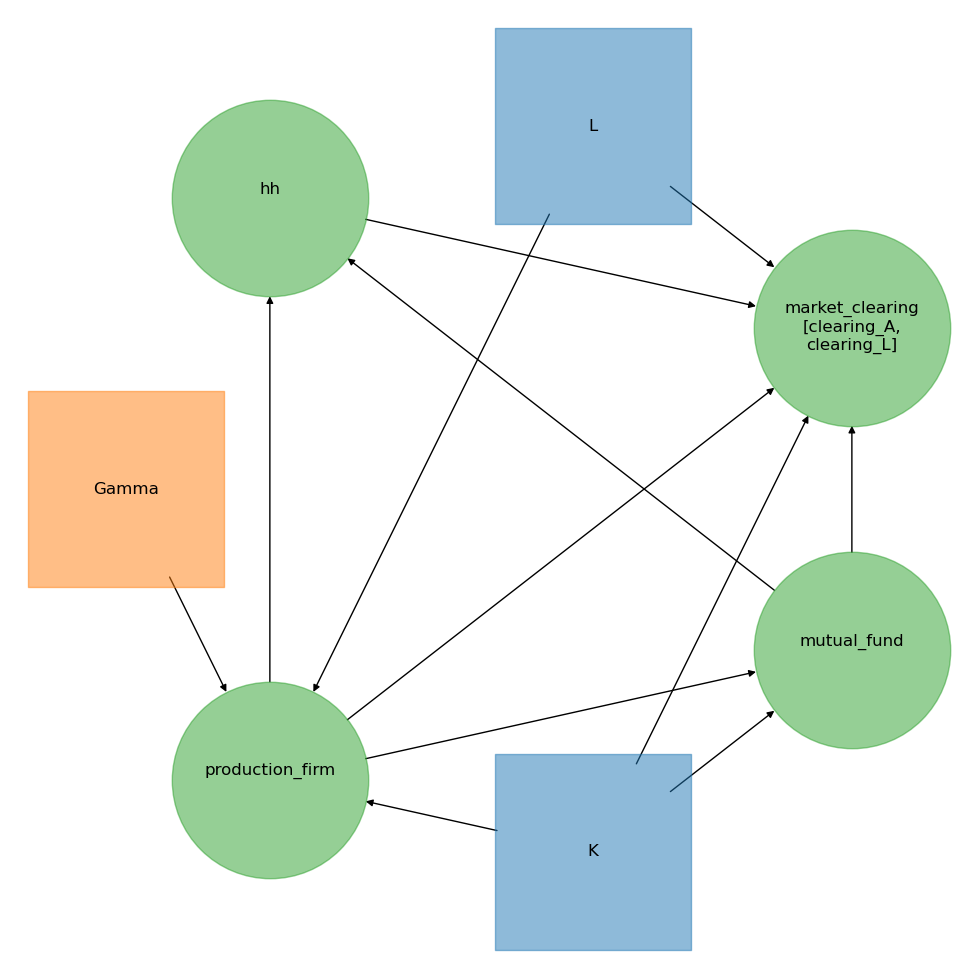
\includegraphics[width=0.4\textwidth]{figs/DAG} 
\begin{itemize}
\item This DAG implies: Exo. input + guess $\Rightarrow$ Firm block $\Rightarrow$
Mutual fund $\Rightarrow$HHs $\Rightarrow$ Residuals 
\end{itemize}
\end{frame}
%
\begin{frame}{Further reduction}
\vspace{-7mm}
\begin{align*}
\boldsymbol{H}\left(\boldsymbol{K},\boldsymbol{\Gamma},\underline{\boldsymbol{D}}_{0}\right) & =\left[\begin{array}{c}
A_{t}-A_{t}^{hh}\\
\forall t\in\{0,1,\dots,T-1\}
\end{array}\right]=\boldsymbol{0}
\end{align*}
where $\boldsymbol{X}=(X_{0},X_{1},\dots,X_{T-1})$, $K_{-1}=\int a_{t-1}d\underline{\boldsymbol{D}}_{0}$
and{\footnotesize{}
\begin{align*}
L_{t} & =1\\
r_{t}^{K} & =\alpha\Gamma_{t}(K_{t-1}/L_{t})^{\alpha-1}\\
w_{t} & =(1-\alpha)\Gamma_{t}(K_{t-1}/L_{t})^{\alpha}\\
A_{t} & =K_{t}\\
r_{t} & =r_{t}^{K}-\delta\\
\boldsymbol{D}_{t} & =\Pi_{z}^{\prime}\underline{\boldsymbol{D}}_{t}\\
\underline{\boldsymbol{D}}_{t+1} & =\Lambda_{t}^{\prime}\boldsymbol{D}_{t}\\
A_{t}^{hh} & =\boldsymbol{a}_{t}^{\ast\prime}\boldsymbol{D}_{t}\\
& \forall t\in\{0,1,\dots,T-1\}
\end{align*}
}\textbf{Truncation:} $T<\infty$ fine when $\Gamma_{t}=\Gamma_{ss}$
for all $t>\underline{t}$ with $\underline{t}\ll T$
\end{frame}
%
\begin{frame}{Solve with Broyden}
\begin{itemize}
\item As with standard Ramsey model from before we have:
\begin{itemize}
\item Equation system with $T$ equations ($\boldsymbol{H}$)
\item And $T$ unknowns ($\boldsymbol{K}$)
\end{itemize}
\item If we can calculate the jacobian of $\boldsymbol{H}$ w.r.t $\boldsymbol{K}$
we can solve with Broyden's method as before
\end{itemize}
\end{frame}
%
\begin{frame}{How to compute Jacobian?}
\begin{itemize}
\item <+->How do we compute the Jacobian of the residuals $\,\boldsymbol{H}$
w.r.t unknowns $\boldsymbol{K}?$
\begin{itemize}
\item Before: Compute Jacobian of entire model using num. diff
\item \textbf{Now}: Use DAG structure + chain rule 
\end{itemize}
\item <+->\emph{Example}. Represent model in block form: \textbf{
\[
\boldsymbol{w},\boldsymbol{r}^{K}=Firm\left(\boldsymbol{K}\right),\quad\boldsymbol{A},\boldsymbol{r}=MutFund\left(\boldsymbol{K},\boldsymbol{r}^{K}\right)
\]
\[
\boldsymbol{A}^{hh}=hh\left(\boldsymbol{r},\boldsymbol{w}\right),\quad\boldsymbol{A}-\boldsymbol{A}^{hh}=\boldsymbol{H}\left(\boldsymbol{A},\boldsymbol{A}^{hh}\right)
\]
}
\item <+->Let $\mathcal{J}^{y,x}$ be Jacobian of $y$ w.r.t $x$. Then:
\begin{align*}
\boldsymbol{H}_{\boldsymbol{K}}\equiv\mathcal{J}^{A-A^{hh},K} & =\mathcal{J}^{A-A^{hh},A}\mathcal{J}^{A,K}\\
& +\mathcal{J}^{A-A^{hh},A^{hh}}\mathcal{J}^{A^{hh},r}\mathcal{J}^{r,r^{k}}\mathcal{J}^{r^{k},K}\\
& +\mathcal{J}^{A_{t}-A^{hh},A^{hh}}\mathcal{J}^{A^{hh},w}\mathcal{J}^{w,K}
\end{align*}
\end{itemize}
\end{frame}
%
\begin{frame}{How to compute Jacobian?}
\begin{itemize}
\item <+->If we have individuals Jacobians, easy to compute $\boldsymbol{H}_{\boldsymbol{K}}$
\begin{itemize}
\item Also very efficient - just matrix mulitiplication \\
\vspace{1cm}
\end{itemize}
\item <+->How to get individual Jacobians?
\begin{itemize}
\item Some are easy: For $\mathcal{J}^{w,K},\mathcal{J}^{r^{k},K}$ we just
have to diff. $r_{t}^{K}=\alpha\Gamma_{t}(K_{t-1}/L_{t})^{\alpha-1},w_{t}=(1-\alpha)\Gamma_{t}(K_{t-1}/L_{t})^{\alpha}$
\begin{itemize}
\item Cheap, and can often be vectorized 
\end{itemize}
\item What about HH Jacobians $\mathcal{J}^{A_{hh},r},\mathcal{J}^{A_{hh},w}$?
\end{itemize}
\end{itemize}
\end{frame}
%
\begin{frame}{Bottleneck: How do we find the Jacobian?}
\begin{itemize}
\item <+->\textbf{Naive approach: }For each input $i$ into HH block $i\in\left\{ r,w\right\} $
\begin{itemize}
\item For each $s\in\{0,1,...,T-1\}$
\begin{enumerate}
\item Shock input $i$ in period $s$ by small amount $\Delta$
\item Solve household problem backwards along transition path
\item Simulate households forward along transition path
\item Calculate column $s$, row $t$ of jacobian as $\frac{\partial\mathcal{J}_{t}^{A_{hh},i}}{\partial i_{s}}=\frac{A_{t}^{hh}-A_{ss}^{hh}}{\Delta}$
for all $t$
\end{enumerate}
\end{itemize}
\textbf{Bottleneck: }We need $T^{2}$ solution steps and simulation
steps for each input $\left\{ r,w\right\} $
\item <+->Solution: \textbf{Fake news algorithm} - only need $T$ steps
(later today)\\
\begin{figure}[H] \centering      
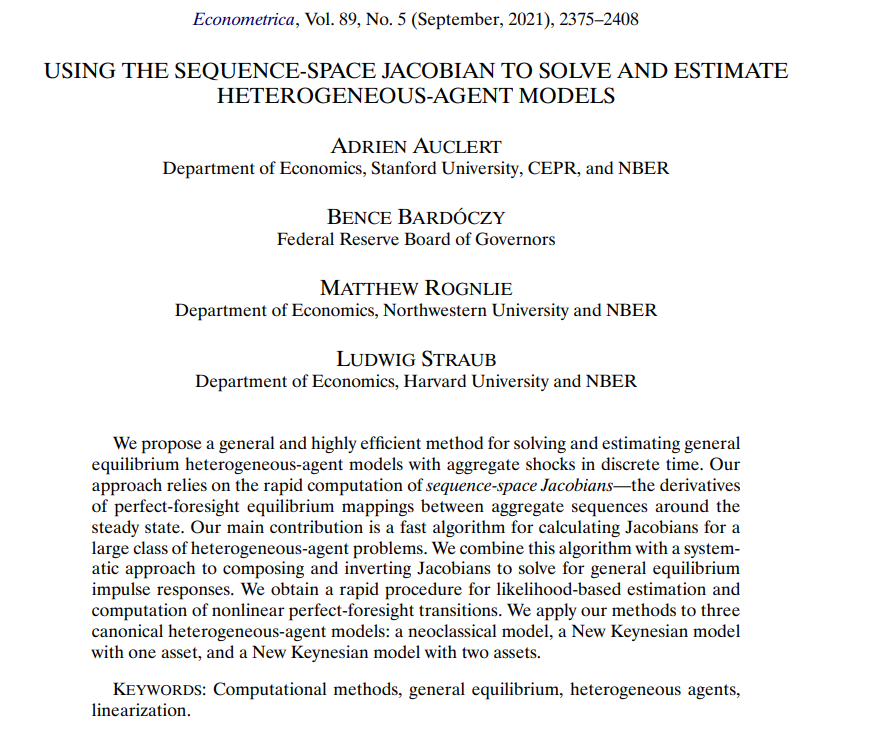
\includegraphics[width=0.3\textwidth]{figs/sequence_space.png}    
\end{figure}
\end{itemize}
\end{frame}
%
\begin{frame}{Summary}
\begin{itemize}
\item Conditional on being able to compute HH jacobian efficiently we can
compute \textbf{transition path }through following steps:
\begin{enumerate}
\item Compute stationary state of model 
\item Formulate transition path as DAG 
\begin{itemize}
\item Reduce number of unknowns and residual equations
\item Not essential, but often good idea 
\end{itemize}
\item Compute Jacobian of residuals $\boldsymbol{H}$ w.r.t unknowns $\boldsymbol{K}$
\item Formulate shock (i.e. TFP increases by 1\% for 4 years)
\item Use Broyden's method to solve for transition path
\end{enumerate}
\end{itemize}
\end{frame}
%
\begin{frame}{Assumptons and interpretation}
\begin{itemize}
\item <+->\textbf{Underlying assumption: }No aggregate uncertainty
\item <+->\textbf{>>Shock<<, $\boldsymbol{\Gamma}$: }A fully unexpected
non-recurrent event $\equiv$ \emph{MIT shock}
\begin{itemize}
\item Unexpected before occuring at time $0$
\item From time $0$ and onwards agents have perfect foresight w.r.t transition
dynamics 
\end{itemize}
\item <+->\textbf{Transition path, $\boldsymbol{K}$: }Non-linear perfect
foresight response to
\begin{enumerate}
\item Initial distribution, $\underline{\boldsymbol{D}}_{0}\neq\boldsymbol{D}_{ss}$or
$K_{0}\neq K_{ss}$ (convergence to steady state)
\item Shock, $\Gamma_{t}\neq\Gamma_{ss}$ for some $t$ (i.e. impulse-response)
\end{enumerate}
\end{itemize}
\end{frame}
%
\begin{frame}{The HANC example from GEModelToolsNotebooks}
\begin{itemize}
\item \textbf{Presentation: }I go through the code
\end{itemize}
\end{frame}
%
\begin{frame}{Interpreting the household Jacobians}
\begin{itemize}
\item \textbf{Jacobian of consumption wrt. wage: }\emph{What happens to
consumption in period $t$ when the wage (and thus income) increases
in period $s$?}\textbf{
\[
\mathcal{J}^{C^{hh},w}=\left[\begin{array}{ccc}
\frac{\partial C_{0}^{hh}}{\partial w_{0}} & \frac{\partial C_{0}^{hh}}{\partial w_{1}} & \cdots\\
\frac{\partial C_{1}^{hh}}{\partial w_{0}} & \ddots & \ddots\\
\vdots & \ddots & \ddots
\end{array}\right]
\]
}
\item \textbf{Columns:} The full dynamic response to a unit shock in period
$s$
\end{itemize}
\end{frame}
%
\begin{frame}{Decomposition of GE response}
\begin{itemize}
\item \textbf{GE transition path:} $\boldsymbol{r}^{\ast}$ and $\boldsymbol{w}^{\ast}$
\item \textbf{PE response of each:}
\begin{enumerate}
\item Set $(\boldsymbol{r},\boldsymbol{w})\in\left\{ \left(\boldsymbol{r}^{\ast},\boldsymbol{w}_{ss}\right),\left(\boldsymbol{r}_{ss},\boldsymbol{w}^{\ast}\right)\right\} $
\item Solve household problem backwards along transition path
\item Simulate households forward along transition path
\item Calculate outcomes of interest
\end{enumerate}
\end{itemize}
\end{frame}
%
\section{Fake News Algorithm}
\begin{frame}{Fake news algorithm}
\begin{itemize}
\item <+->\textbf{Household block:} 
\begin{align*}
\boldsymbol{Y}^{hh} & =hh(\boldsymbol{X}^{hh})
\end{align*}
\begin{itemize}
\item i.e. $\boldsymbol{Y}^{hh}=C^{hh},A^{hh}$ and $\boldsymbol{X}^{hh}=w,r$
\end{itemize}
\item <+->\textbf{Goal:} Fast computation of
\[
\mathcal{J}^{hh,}=\frac{dhh(\boldsymbol{X}_{ss}^{hh})}{d\boldsymbol{X}^{hh}}
\]
\item <+->\textbf{Naive approach:} 
\begin{itemize}
\item Shock at time $s=0$, solve + simulate HH block for $T$ periods
\item Repeat until $s=T-1$
\item Requires $T^{2}$ solution and simulation steps 
\end{itemize}
\item <+->\textbf{Next slides: }\emph{Sketch of much faster approach}
\end{itemize}
\end{frame}
%
\begin{frame}{Initial step}
\begin{itemize}
\item Note that aggregate is (matrix) product of individual policy function
$\boldsymbol{y}_{t}$ and distribution $\boldsymbol{D}_{t}$. 
\item Linearize (first-order Taylor) around ss:
\begin{align*}
\boldsymbol{Y}^{hh} & =\left(\boldsymbol{y}_{t}'\right)\boldsymbol{D}_{t}\\
\Rightarrow\frac{d\boldsymbol{Y}^{hh}}{d\boldsymbol{X}^{hh}} & =\left(\frac{d\boldsymbol{y}_{t}}{d\boldsymbol{X}^{hh}}'\right)\boldsymbol{D}_{ss}+\left(\boldsymbol{y}_{ss}'\right)\frac{d\boldsymbol{D}_{t}}{d\boldsymbol{X}^{hh}}
\end{align*}
\item What can we say about policy function term $d\boldsymbol{y}_{t}$?
\end{itemize}
\end{frame}
%
\begin{frame}{Pertubation of policy function}
\begin{itemize}
\item <+->The heart of the fake news algorithm is a central insight that
allow us to compute $d\boldsymbol{y}_{t}/d\boldsymbol{X}^{hh}$ efficiently
\item <+->Let $\boldsymbol{y}_{t}^{s}$ be policy function at time $t$
following a shock in period $s$. Then:
\[
\boldsymbol{y}_{t}^{s}=\begin{cases}
\boldsymbol{y}_{ss} & t>s\\
\boldsymbol{y}_{t+j}^{s+j} & t\leq s
\end{cases}
\]
\item <+->Verbally: The response of the policy function $\boldsymbol{y}$
at time $t$ to a shock at $s$ is the as the response at time $t+j$
to a shock at $s+j$
\begin{itemize}
\item Policy function \textbf{does not depend on the absolut time of shock}
only the relative distance between >>today<< and the shock, $s-t$.
\end{itemize}
\item <+->\textbf{Implication}: We need to only do a single backwards iteration
to a shock at $s=T-1$. 
\begin{itemize}
\item Can then construct change in policy function $d\boldsymbol{y}_{t}^{s}/d\boldsymbol{X}^{hh}$
for different $s$ by shifting policy function around 
\end{itemize}
\end{itemize}
\end{frame}
%
\begin{frame}{Numerical illustration}
Graphically. Response of $c_{t}$ to income shock at $s=3,5$\\
\begin{figure}[H]  
\centering 
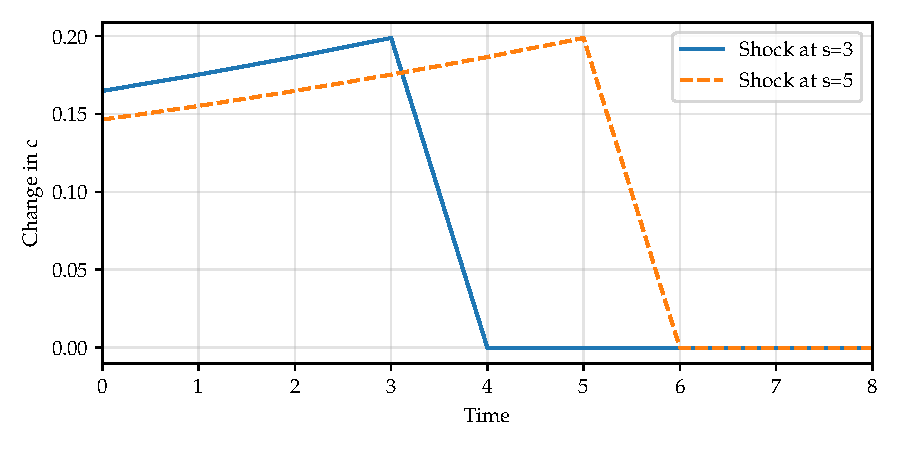
\includegraphics[width=0.6\linewidth]{figs/irf_fakenews1.pdf} 
\end{figure}
\begin{figure}[H]  
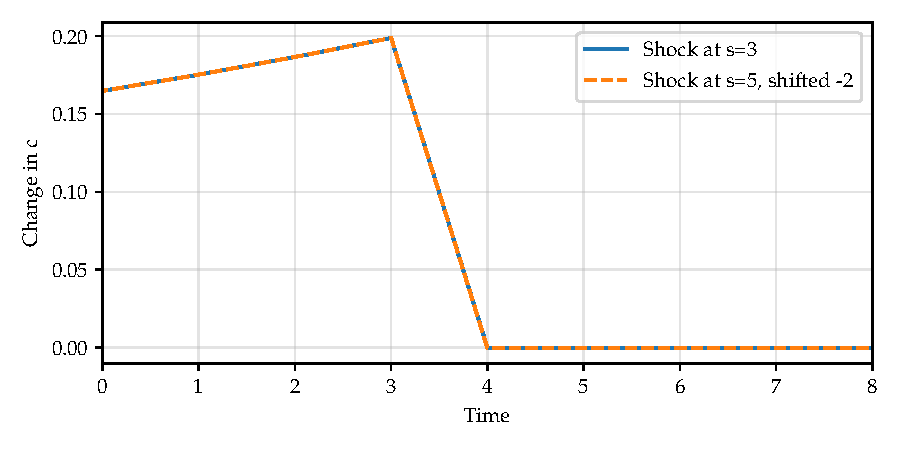
\includegraphics[width=0.6\linewidth]{figs/irf_fakenews2.pdf} 
\end{figure}
\end{frame}
%
\begin{frame}{Aggregate Jacobian }
\begin{itemize}
\item <+->Can we use same logic for aggreregate Jacobian, $\mathcal{J}_{t,s}=\mathcal{J}_{t-1,s-1}$?
\begin{itemize}
\item No - the above is true for \emph{policy} function, but not \textbf{distribution}
\item Distribution is backwards looking ($\boldsymbol{D}_{t}^{s}=\left(\boldsymbol{\Lambda}_{t}^{s}\Pi_{ss}\right)'\boldsymbol{D}_{t-1}^{s}$)
so number of periods $t$ since announcement matters
\end{itemize}
\item <+->Can write aggregate Jacobian as:
\[
\mathcal{J}_{t,s}=\begin{cases}
\mathcal{F}_{t,s} & \text{ for }t=0,s=0\\
\mathcal{J}_{t-1,s-1}+\mathcal{F}_{t,s} & \text{ for }t,s>0
\end{cases}
\]
\item <+->where $\mathcal{F}_{t,s}$ is the \textbf{fake news} matrix.
\item <+->Element $\left(t,s\right)$ in matrix $\mathcal{F}$ for $t>0$
is 
\begin{align*}
\mathcal{F}_{t,s}= & \left(\boldsymbol{y}_{ss}\right)'\left(\boldsymbol{\Lambda}'_{ss}\right)^{t}\frac{d\boldsymbol{D}_{1}^{s}}{d\boldsymbol{X}^{hh}}
\end{align*}
\item <+->Why >>fake news<<? $\mathcal{F}_{t,s}$ captures effect of
announcing a date$-s$ shock at time $0$, and retracting the annountment
at date 1
\begin{itemize}
\item Policy variables revert to steady state after period 1, but distribution
changes since $d\boldsymbol{y}_{0}\neq0$
\end{itemize}
\end{itemize}
\end{frame}
%
\begin{frame}{Fake News Matrix}
\begin{itemize}
\item <+->Can show that the fake news matrix can be computed as:
\[
\mathcal{F}_{t,s}\equiv\begin{cases}
\left(\frac{d\boldsymbol{y}_{0}^{s}}{d\boldsymbol{X}^{hh}}\right)'\boldsymbol{D}_{ss} & t=0\\
\left(\boldsymbol{y}_{ss}\right)'\left(\boldsymbol{\Lambda}'_{ss}\right)^{t}\frac{d\boldsymbol{D}_{1}^{s}}{d\boldsymbol{X}^{hh}} & t>0
\end{cases}
\]
\item <+->$t=0$ element: Easy to compute when we have $d\boldsymbol{y}_{0}^{s}/d\boldsymbol{X}^{hh}$
\begin{itemize}
\item Can get this from a single backwards run ($T$ periods) due to logic
from before 
\end{itemize}
\item <+->$t>0$ elements: Only involves basic matrix multiplication once
we have $d\boldsymbol{D}_{1}^{s}/d\boldsymbol{X}^{hh}$
\begin{itemize}
\item Since we have derivatves of policy function for all $t,s$ $d\boldsymbol{y}_{t}^{s}/d\boldsymbol{X}^{hh}$
can get $d\boldsymbol{D}_{1}^{s}/d\boldsymbol{X}^{hh}$ easily
\item Note: Not too expensive since histogram method for distribution is
fast and efficient 
\end{itemize}
\end{itemize}
\end{frame}
%
\begin{frame}{Fake news algorithm - summary}
\begin{itemize}
\item <+->Auclert et. al (2021) introduce an efficient alogirthm to compute
aggregate jacobians for models with heterogeneous agents 
\begin{itemize}
\item Can compute the linearized response of aggregate consumption, savings
w.r.t aggregate variables such as wages, interest rates \textbf{fast}
\end{itemize}
\item <+->Central insight: Exploit structure of dynamic programming problems
+ histogram method 
\item <+->Why did we need this? 
\begin{itemize}
\item Allows us to compute Jacobian of aggregate model by >>chaining<<
together individual jacobians along DAG
\item Can then use Quasi-Newton methods to solve dynamic GE model
\end{itemize}
\item <+->GEModeltools does all of this >>under the hood<< when you compute
HH Jacobians
\begin{itemize}
\item You just tell GEModeltools the inputs and outputs of the household
block 
\item Entire algorithm is automated 
\end{itemize}
\end{itemize}
\end{frame}
%
\section{Exercises}
\begin{frame}{Exercises: HANCGovModel}
Same model. Your choice of $\tau_{ss}.$ New questions:
\begin{enumerate}
\item \textbf{Define the transition path.}
\item \textbf{Plot the DAG}
\item \textbf{What do the Jacobians look like?}
\item \textbf{Find the transition path for $G_{t}=G_{ss}+0.01G_{ss}0.95^{t}$}
\item \textbf{What explains household savings behavior?}
\item \textbf{What happens to consumption inequality?}
\end{enumerate}
\end{frame}
%
\section{Summary}
\begin{frame}{Summary and next week}
\begin{itemize}
\item \textbf{Today: }
\begin{enumerate}
\item The concept of a transition path
\item Details of the \textcolor{DarkRed}{\href{https://github.com/NumEconCopenhagen/GEModelTools}{GEModelTools}}
package
\end{enumerate}
\item \textbf{Homework:} Work on completing the model extension exercise
\item \textbf{Next week: }Begin working on Assignment 1
\end{itemize}
\end{frame}
%
\end{document}
